\chapter{Resultados}

\section{Manual de uso de la base de datos}

A continuación, se enseñarán los pasos necesarios para una correcta utilización de la base de datos. Esta sección del documento está indicada para todo aquel que participe en el desarrollo del proyecto.

Para acceder a la consola de control de MongoDB es necesario localizar el identificador del contenedor de docker de Mongo dentro de la máquina donde se haya realizado el despliegue. Esto es posible mediante el comando \textbf{docker ps -a}, que listará todos los contenedores levantados en la máquina. Sólo es necesario recordar los tres primeros caracteres del contenedor. Una vez tengamos el identificador, introducimos el siguiente comando en un terminal, \textbf{docker exec -t 'identificador' bash}. Con el último parámetro indicamos que queremos abrir un terminal dentro del contenedor y como indicador podemos introducir los tres caracteres mencionados anteriormente. Esto provocará que cambie el prompt de la consola al prompt del contenedor. Posteriormente introducimos el comando \textbf{mongo} que abrirá el cliente de línea de comandos de mongo. 

Primeramente tenemos que acceder a la base de datos con la que queremos interactuar, esto se consigue mediante el comando \textbf{use SonidosDelCielo}.

Después introducimos los credenciales necesarios de la siguiente forma:
\newline\textbf{db.auth('usuario','contraseña')}. Esta operación retornará 1 en caso de ser correcta o 0 en cualquier otro caso.

Una vez estemos logueados dentro de la base de datos, podremos realizar varios tipos de operaciones.


\subsection{Inserción en colección}

Cuando ya estemos dentro del terminal de mongo, tenemos que introducir los siguientes comandos:

\begin{itemize}
    \item \textbf{db.collection.insert(documento)}: es necesario sustituir el parámetro <collection> por cualquier colección que esté declarada previamente, en nuestro caso (Eco, Estacion, Usuario, Espectrograma, Curva Luz, Sonido y Clasificacion) y como documento se introduce un fichero en formato JSON.
\end{itemize}

En caso de producirse una inserción correcta, retornará un JSON con el par clave-valor \{"nInserted", <número>\}, siendo número la cantidad de documentos insertados correctamente. En la siguiente imagen \ref{fig:insertMongo} se puede ver el proceso completo de inserción correcta.

\begin{figure}[h]
    \centering
    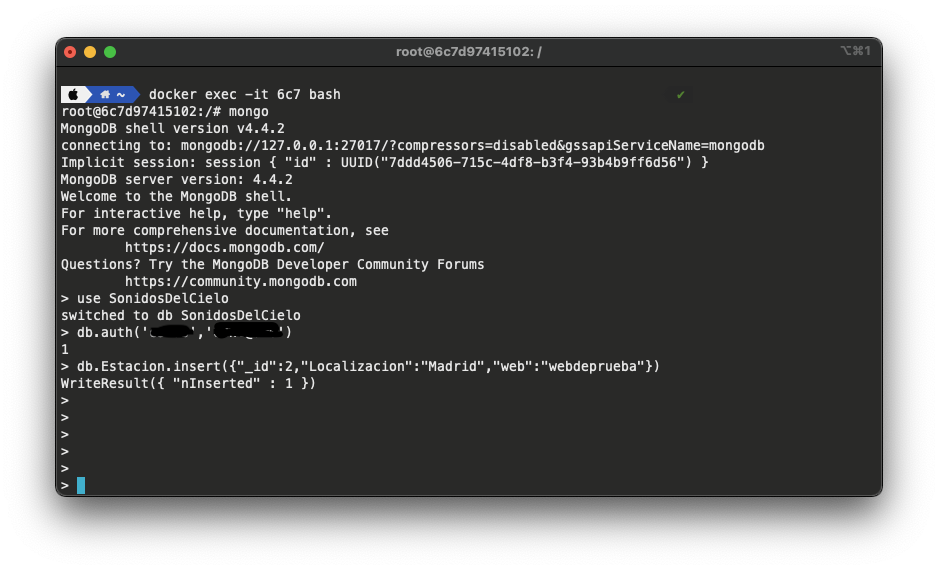
\includegraphics[width=0.8\textwidth]{include/resultados/InsertMongo.png}
    \caption{Inserción en el terminal de MongoDB}
    \label{fig:insertMongo}
\end{figure}

\subsection{Obtención de un documento}

Para la obtención del documento, una vez estemos ubicados y logueados dentro de la base de datos indicada, solamente será necesario introducir el siguiente comando: \textbf{db.getCollection('Coleccion').find(JSON)}.

Dentro del JSON podemos colocar la cantidad de filtros que consideremos necesarios. En este caso hemos introducido el filtro de Localizacion dentro de la colección Estacion, como podemos ver en la imagen \ref{fig:findMongo}. Si hay algún documento que satisfaga esos filtros, se retornará un JSON con los diferentes documentos, en caso de no existir ninguno, el retorno estará vacío.

\begin{figure}[h]
    \centering
    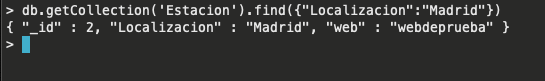
\includegraphics[width=0.8\textwidth]{include/resultados/FindMongo.png}
    \caption{Obtención de documento en el terminal de MongoDB}
    \label{fig:findMongo}
\end{figure}


\subsection{Modificación de un documento}

Para realizar la actualización de un documento en MongoDB es muy sencilla, simplemente tenemos que introducir el comando \textbf{db.collection.updateOne(filter, update)} con los filtros que queramos y como update un documento JSON con los diferentes parámetros a añadir o modificar, ya que en este tipo de bases de datos no es necesario que todos los documentos tengan la misma estructura, podemos ver un ejemplo de actualización en la figura \ref{fig:update_Mongo}.

\begin{figure}[h]
    \centering
    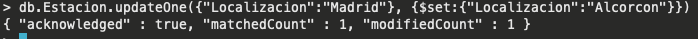
\includegraphics[width=0.8\textwidth]{include/resultados/UpdateMongo.png}
    \caption{Modificación de documento en el terminal de MongoDB}
    \label{fig:update_Mongo}
\end{figure}


MongoDB también nos permite actualizar varios documentos que cumplan con los filtros introducidos a través del comando \textbf{db.collection.updateMany(filter, update)}

\subsection{Eliminación de un documento}

En caso de querer eliminar todos los documentos existentes dentro de la colección, introduciremos el comando \textbf{db.Coleccion.deleteMany({})} y como parámetro un JSON vacío. Si sólo queremos eliminar un documento debemos introducir el mandato \textbf{db.Coleccion.deleteOne({JSON})} y dentro del JSON pasaremos los filtros adecuados para la eliminación del documento, como se muestra en la figura \ref{fig:deleteMongo}.

\begin{figure}[h]
    \centering
    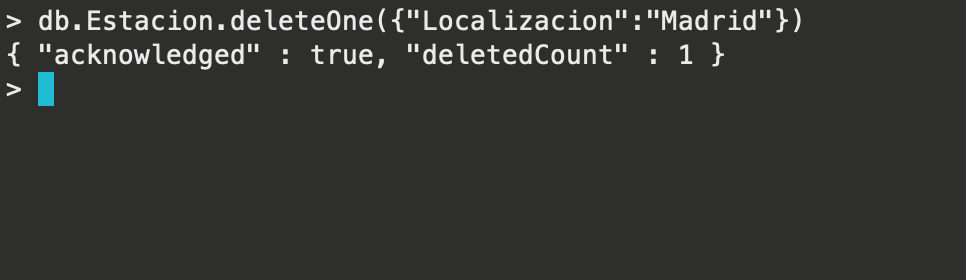
\includegraphics[width=0.8\textwidth]{include/resultados/DeleteMongo.png}
    \caption{Eliminación de un documento en el terminal de MongoDB}
    \label{fig:deleteMongo}
\end{figure}


\section{Manual de uso de la API}

Con el desarrollo de la API RESTful se incluyó la herramienta Swagger. Esta herramienta permite realizar pruebas sobre los distintos recursos implementados. En nuestro caso se han implementado 4 operaciones sobre cada recurso existente (Eco, Estación, Curva de Luz, Espectrograma, Clasificacion y Usuario) como se ha mostrado en la figura \ref{fig:swagger_ui}. Estas cuatro operaciones son:

\begin{enumerate}
    \item Get: obtención de un recurso.
    \item Put: creación de un nuevo recurso.
    \item Patch: modificación sobre un recurso existente. Utilizamos la operación Patch sobre Put debido al funcionamiento de MongoDB. Si utilizamos PUT, MongoDB nos obliga a modificar el id del recurso.
    \item Delete: eliminación de un documento.
\end{enumerate}

Vamos a mostrar cómo se realiza cada una de las anteriores operaciones sobre la interfaz de swagger. Además gracias a la utilización de la herramienta, nos brinda el comando equivalente para utilizar desde un terminal. 

\subsection{Utilización del método GET}

Cada uno de los recursos se ha dotado de 2 operaciónes GET. La primera de ellas y sin la introducción de un identificador nos devuelve un documento JSON con todos los elementos disponibles que existan. En cambio, si introducimos un identificador como parámetro, obtendremos un solo elemento, como se muestra en la siguiente figura \ref{fig:swagger_get}. 

\begin{figure}[h]
    \centering
    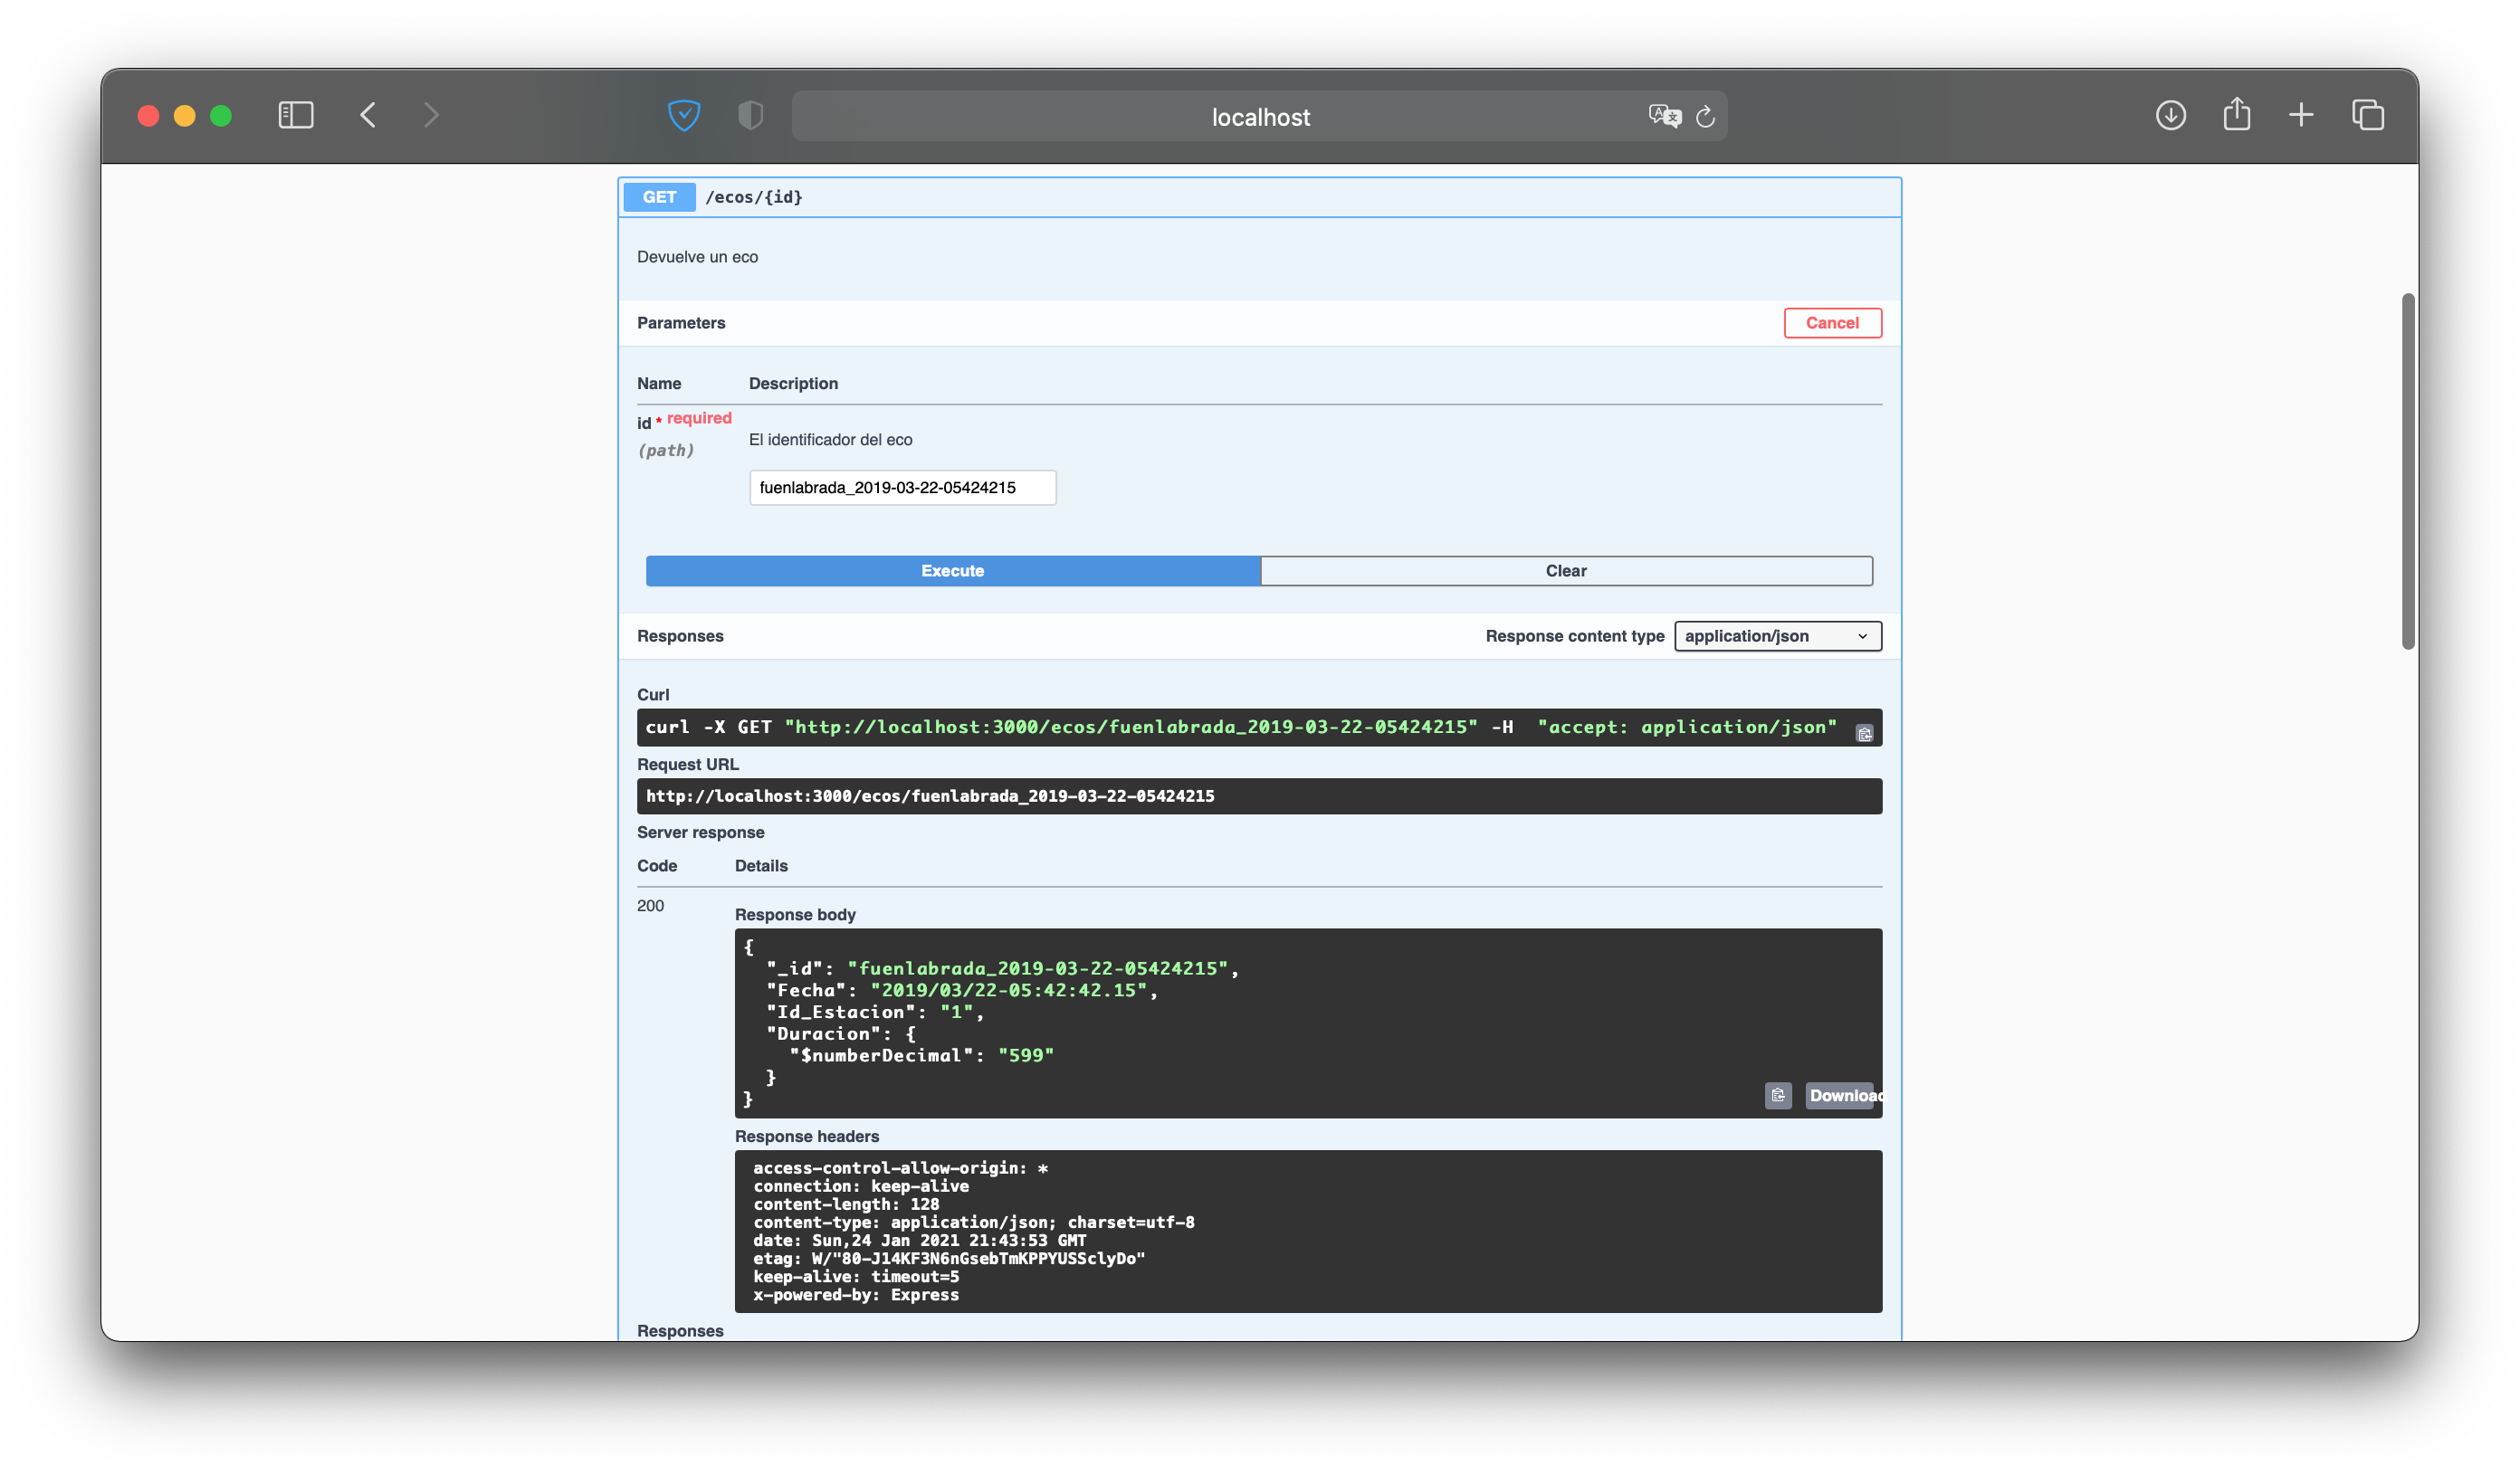
\includegraphics[width=\textwidth]{include/resultados/SwaggerGet.png}
    \caption{Obtención de un recurso por medio de Swagger}
    \label{fig:swagger_get}
\end{figure}

Se observa cómo la herramienta nos proporciona el código que devuelve el response (200 en este caso) y un JSON con el recurso.

\subsection{Utilización del método POST}

Para el uso del método POST se ha implementado una vista de cada uno de los recursos de forma que es visible en todo momento el formato que debe seguir el JSON. En este ejemplo vamos a introducir una nueva estación para lo cual se especifica que el formato a seguir es el siguiente:

\begin{lstlisting}
{
  "_id": "string",
  "Localizacion": "string",
  "web": "string"
}
\end{lstlisting}

Para realizar una inserción, simplemente se realiza la modificación del JSON y pulsamos el botón \textit{Execute}. Puesto que MongoDB no es estricto en el formato de los documentos, podemos introducir nuevos campos o incluso reducir los mismo siempre y cuando exista un ''\_id'', tal y como se ve en la figura \ref{fig:swagger_post}.

\begin{figure}[H]
    \centering
    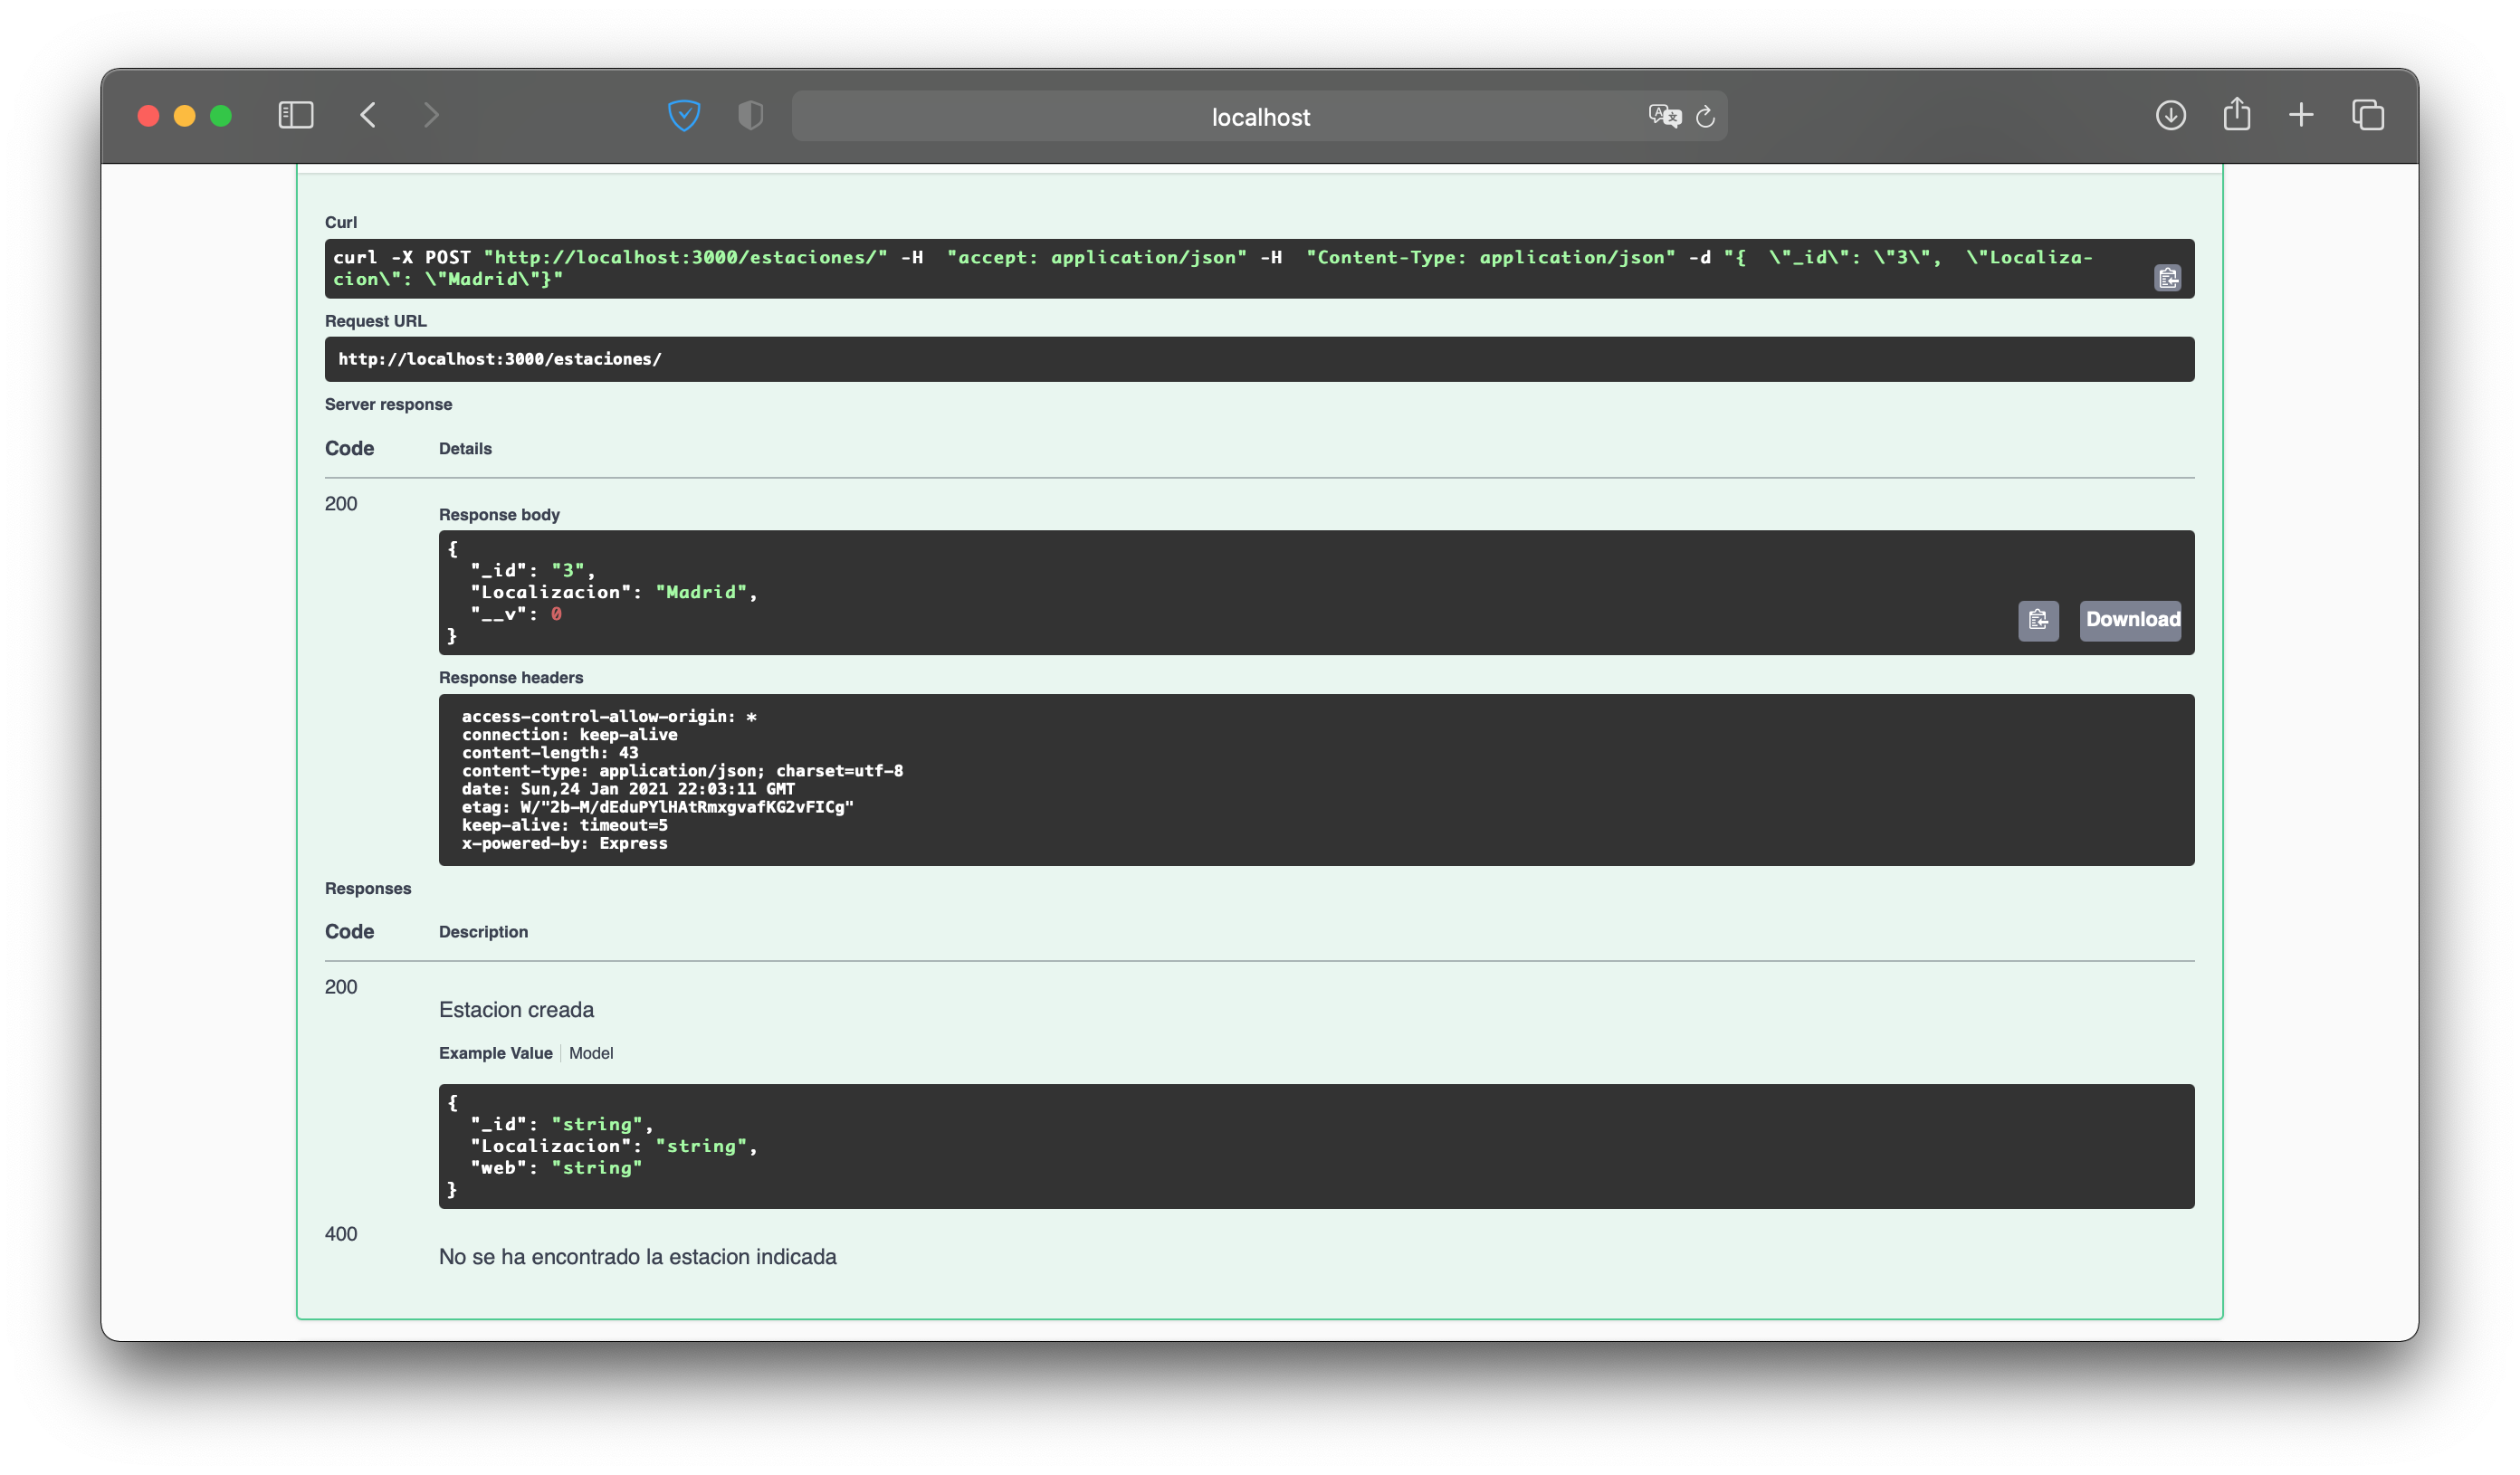
\includegraphics[width=\textwidth]{include/resultados/SwaggerPost.png}
    \caption{Inserción de un recurso por medio de Swagger}
    \label{fig:swagger_post}
\end{figure}

En este caso el código de respuesta es un 200 con el texto ''Estacion creada''.

Puesto que dentro del proyecto Sonidos del Cielo existen ciertas tareas que se realizan de manera periódica, se ha desarrollado un pequeño programa en lenguaje Python, que sirve para la inserción automática de los elementos que se generan a través del programa Echoes (ecos, espectrogramas, curva de luz) y sonidos generados mediante el programa desarrollado por el equipo del CSLab. El programa se encarga de leer un fichero csv, selecciona las columnas necesarias para cada elemento y tantas peticiones POST como líneas existan en el programa. En la siguiente figura \ref{fig:insert_script} se muestra uno de los métodos utilizados

\begin{figure}[H]
    \centering
    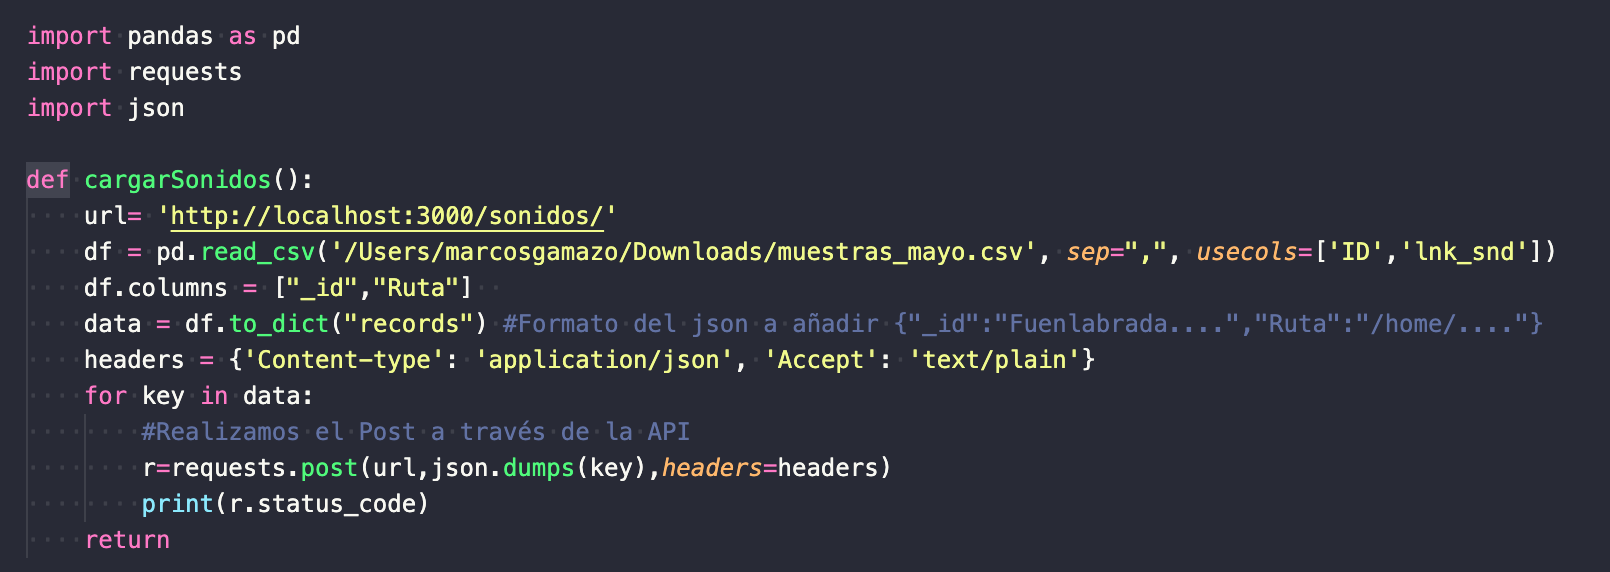
\includegraphics[width=\textwidth]{include/resultados/InsertScript.png}
    \caption{Inserción a través del script en Python}
    \label{fig:insert_script}
\end{figure}

De esta forma y mediante un comando cron, es posible añadir todos los elementos que se detecten diariamente.

\subsection{Utilización del método Patch}

Para utilizar este método es necesario introducir como parámetro el id del recurso a modificar y posteriormente dentro del body las modificaciones pertinentes que se deseen realizar. En caso de introducir otro id, el programa lo eliminará y realizará los cambios sobre el id que se ha pasado como \textit{Path Param}. El proceso de modificación es similar al de inserción, se muestra un JSON como referencia al modelo que debemos introducir y al igual que en el método anterior, podemos añadir, eliminar o actualizar datos de un recurso existente.

\subsection{Utilización del método Delete}

Para la eliminación de un recurso, simplemente lo único que necesitamos es el identificador del recurso que queremos borrar. En caso de que el recurso exista, la API retornará un response con código 200 y el elemento que existía con ese identificador antes de ser eliminado, como se muestra en la figura \ref{fig:swagger_delete}

\begin{figure}[H]
    \centering
    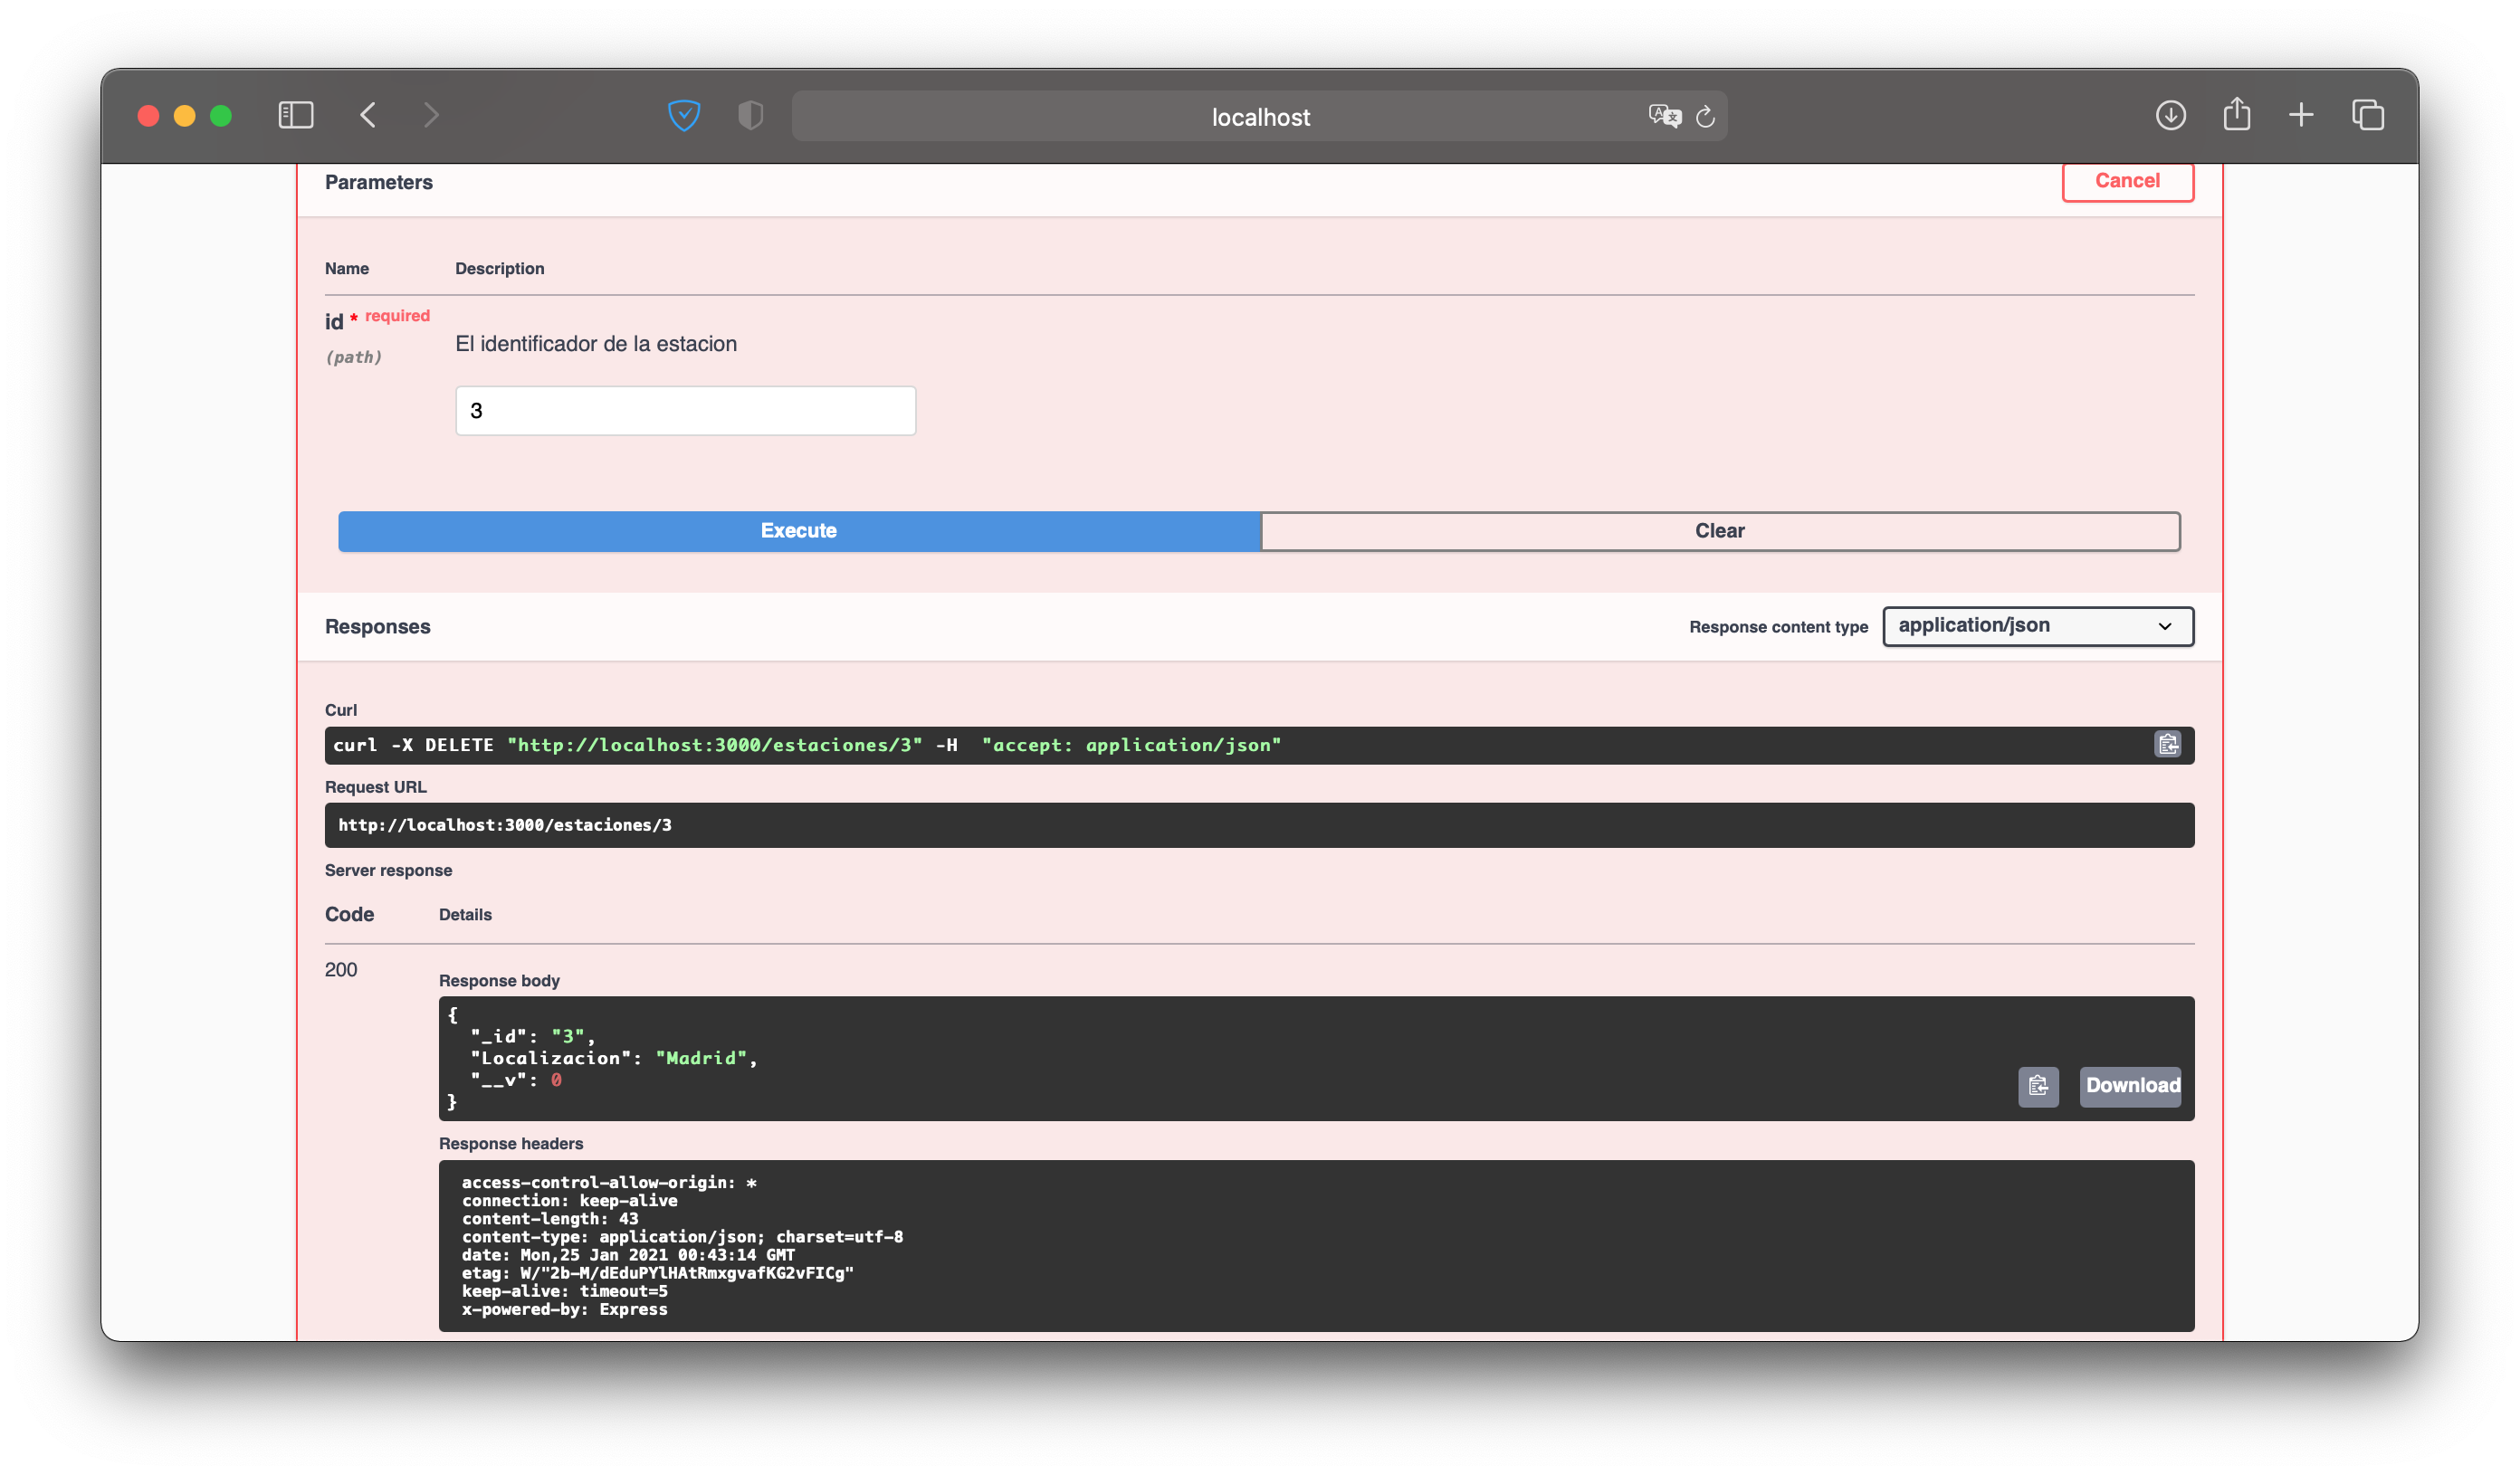
\includegraphics[width=\textwidth]{include/resultados/SwaggerDelete.png}
    \caption{Eliminación de un recurso por medio de Swagger}
    \label{fig:swagger_delete}
\end{figure}


\newpage
\section{Manual de uso del Chatbot}

El chatbot se ha desarrollado para corroborar el correcto funcionamiento de la API RESTful. A continuación se explicará paso a paso y con imágenes la utilización del mismo. Una vez se hayan puesto en funcionamiento ambos servidores de Rasa

En primer lugar en la página principal de la web, tenemos un pequeño circulo en la esquina inferior izquierda con un efecto de parpadeo. Una vez pulsemos en el icono en el que aparece un pájaro, aparecerá un cuadro en el que se puede introducir texto. Para que el chatbot comience a funcionar es necesario que introduzcamos un saludo como se muestra en la imagen \ref{fig:init_rasa}.

\begin{figure}[H]
    \centering
    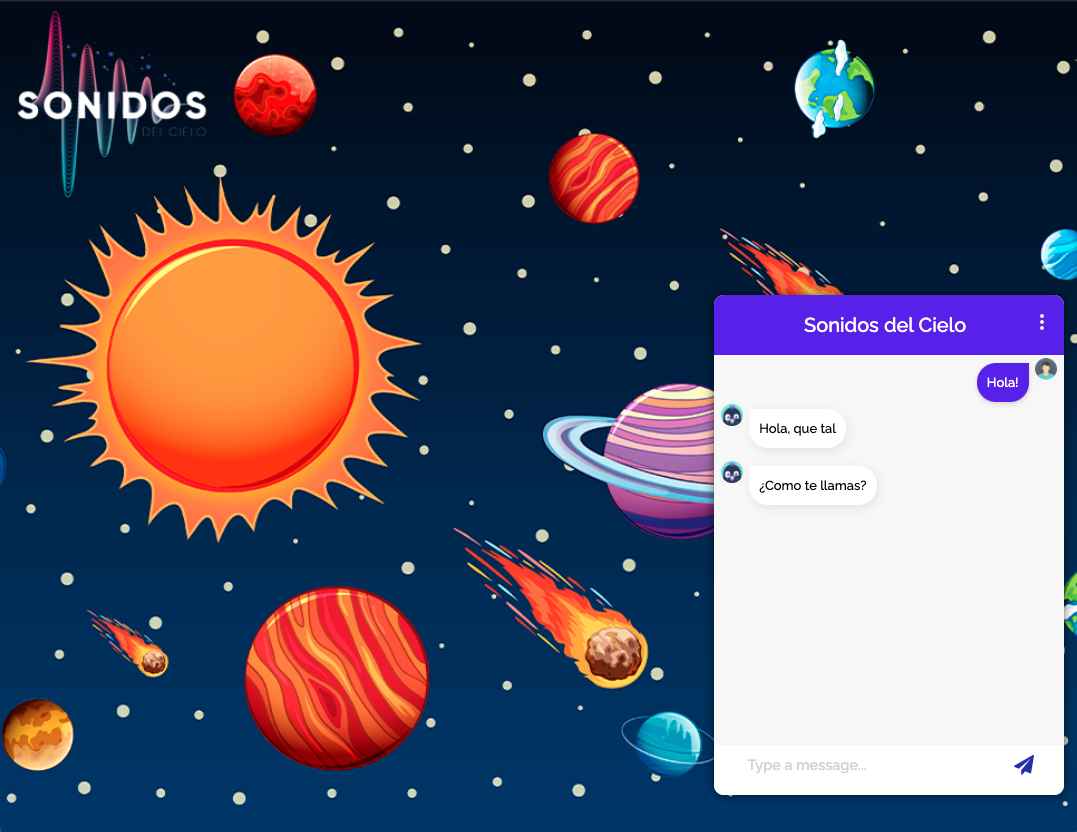
\includegraphics[width=0.7\textwidth]{include/resultados/RasaInit.png}
    \caption{Comienzo de una conversación con el chatbot}
    \label{fig:init_rasa}
\end{figure}

Después el chatbot preguntará el nombre al usuario, en caso de proporcionarlo, se utilizará esta información para almacenar la clasificación. Posteriormente el chatbot mostrará las distintas opciones disponibles, puesto que está enfocado a un público infantil. Se mostrarán cuatro botones para que no sea necesario el uso de la escritura para la interacción con el chatbot. Estos cuatro botones contienen las diferentes opciones a realizar en el chatbot tal y como se ve en la figura \ref{fig:rasa_options}

\begin{itemize}
    \item Tutorial: Muestra una breve explicación sobre el proceso que tiene que seguir el usuario para clasificar un eco.
    \item ¿Qué es el proyecto Sonidos del Cielo?: proporciona un enlace para acceder a la página web del proyecto.
    \item Clasificar: para iniciar la clasificación de un Eco.
    \item Salir: finaliza el programa.
\end{itemize}

\begin{figure}[H]
    \centering
    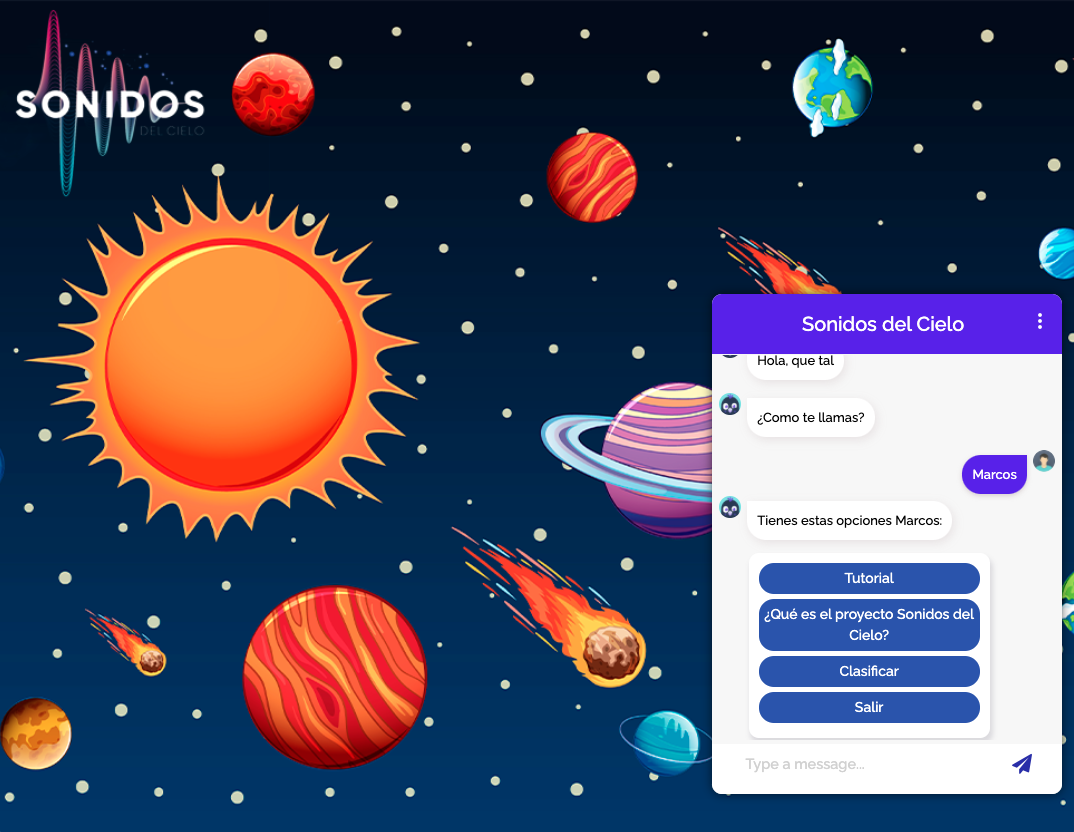
\includegraphics[width=0.7\textwidth]{include/resultados/RasaOptions.png}
    \caption{Muestra de opciones del chatbot}
    \label{fig:rasa_options}
\end{figure}

Una vez pulsemos en la opción de \textbf{Clasificar} se mostrará un reproductor de audio con el sonido del eco y una primera pregunta utilizada para la clasificación.

\begin{figure}[H]
    \centering
    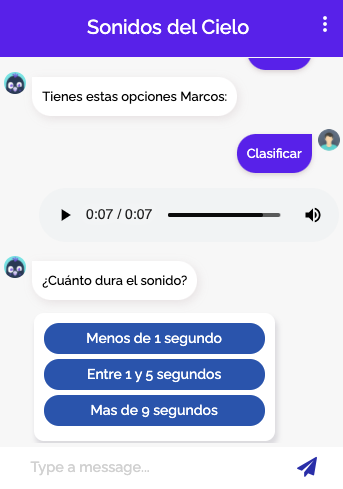
\includegraphics[scale=0.6]{include/resultados/RasaPrimeraPregunta.png}
    \caption{Muestra de sonido y primera pregunta}
    \label{fig:primera_pregunta}
\end{figure}

Una vez respondamos a la pregunta, se nos mostrarán dos preguntas más de la misma forma que se observa en la figura \ref{fig:primera_pregunta}. Cuando se contesten las tres preguntas, el chatbot internamente llamará a un action personalizado que realizará la petición POST a la API y de esta forma se almacenará la clasificación realizada por el usuario. Una vez acabado, volverá a mostrar las distintas opciones del chatbot (figura \ref{fig:init_rasa}) para que en caso de que el usuario quiera, pueda clasificar más sonidos.